\documentclass[a4paper]{article}
\usepackage[a4paper,margin=0mm]{geometry}
\usepackage{fontspec}
\usepackage{unicode-math}
\usepackage{tikz}
\usepackage[table]{xcolor}
\usepackage[absolute]{textpos}
\usepackage{array}
\usepackage{multirow}

\setmainfont{Libertinus Serif}
\setsansfont{Libertinus Sans}
\setmathfont{Libertinus Math}

\definecolor{accent}{HTML}{0F6A52}
\definecolor{badge}{HTML}{A9CFC2}
\definecolor{ink}{HTML}{2A2E30}

\setlength{\TPHorizModule}{1mm}
\setlength{\TPVertModule}{1mm}
\setlength{\parindent}{0pt}
\setlength{\parskip}{0pt}
\emergencystretch=3em
\abovedisplayskip=4pt plus 2pt minus 2pt \belowdisplayskip=4pt plus 2pt minus 2pt \abovedisplayshortskip=2pt \belowdisplayshortskip=2pt
\pagestyle{empty}
\binoppenalty=10000

\newcommand{\LCOL}{16mm}
\newcommand{\RCOL}{111mm}
\newcommand{\COLW}{83mm}

\newcommand{\topicheader}[2]{%
\begin{textblock*}{194mm}(16mm,10mm)
\begin{tikzpicture}
\node[fill=accent,text=white,font=\sffamily\bfseries\fontsize{13}{13}\selectfont,
      minimum width=9mm,minimum height=9mm,inner sep=0pt] at (4.5mm,-4.5mm) {#1};
\node[font=\sffamily\bfseries\fontsize{15}{16}\selectfont,text=ink,anchor=west] at (12mm,-4.5mm) {#2};
\end{tikzpicture}
\end{textblock*}
\begin{textblock*}{194mm}(16mm,22.5mm)

\begin{tikzpicture}
\fill[accent] (0,0) rectangle (194mm,0.5mm);
\end{tikzpicture}
\end{textblock*}
}

\newcommand{\pagefooter}[1]{%
\begin{textblock*}{194mm}(8mm,286.41mm)
  
\begin{tikzpicture}
    \fill[accent] (0,0) rectangle (194mm,0.6mm);
  \end{tikzpicture}
\end{textblock*}
\begin{textblock*}{63.59mm}(8mm,288.27mm)
  {\sffamily\bfseries\color{accent}\fontsize{13}{16}\selectfont SAT 1200+}
\end{textblock*}
\begin{textblock*}{10mm}(188mm,288.27mm)
  \centering{\sffamily\color{accent}\fontsize{14}{16}\selectfont #1}
\end{textblock*}
}

\newcommand{\colrule}[2]{%
\begin{textblock*}{1mm}(105mm,#1mm)
\begin{tikzpicture}
\draw[black!65,line width=0.5pt] (0,0) -- (0,#2mm);
\end{tikzpicture}
\end{textblock*}
}

\newcommand{\setkicker}[2]{%
{\sffamily\bfseries\fontsize{12}{14}\selectfont #1.}\ {\itshape\fontsize{11}{14}\selectfont\color{black!75} #2}\par\vspace{2mm}%
}

\setlength{\fboxsep}{1.4pt}
\setlength{\fboxrule}{0.5pt}
\newcommand{\pnum}[1]{\fcolorbox{ink}{white}{\sffamily\bfseries\fontsize{8}{8}\selectfont #1}~}

% ---- SAT-style multiple-choice block (2x2 grid of short choices) ----
\newcommand{\satq}[6]{%
\noindent\pnum{#1} #2\par\nobreak\vspace{2mm}%
\noindent\hspace*{7mm}\begin{tabular}[t]{@{}p{32mm}p{32mm}@{}}
(A) #3 & (B) #4 \\[2mm]
(C) #5 & (D) #6 \\
\end{tabular}\par\vspace{4.2mm}%
}

% ---- stacked choices for long ones ----
\newcommand{\satqw}[6]{%
\noindent\pnum{#1} #2\par\nobreak\vspace{2mm}%
\noindent\hspace*{7mm}(A) #3\par\vspace{1.6mm}%
\noindent\hspace*{7mm}(B) #4\par\vspace{1.6mm}%
\noindent\hspace*{7mm}(C) #5\par\vspace{1.6mm}%
\noindent\hspace*{7mm}(D) #6\par\vspace{4.2mm}%
}

% ---- automatic choice: 2x2 grid when every choice is short, stacked otherwise ----
\newsavebox{\chA}\newsavebox{\chB}\newsavebox{\chC}\newsavebox{\chD}
\newcommand{\satqa}[6]{%
\sbox{\chA}{#3}\sbox{\chB}{#4}\sbox{\chC}{#5}\sbox{\chD}{#6}%
\ifdim\wd\chA>26mm \satqw{#1}{#2}{#3}{#4}{#5}{#6}\else
\ifdim\wd\chB>26mm \satqw{#1}{#2}{#3}{#4}{#5}{#6}\else
\ifdim\wd\chC>26mm \satqw{#1}{#2}{#3}{#4}{#5}{#6}\else
\ifdim\wd\chD>26mm \satqw{#1}{#2}{#3}{#4}{#5}{#6}\else
\satq{#1}{#2}{#3}{#4}{#5}{#6}\fi\fi\fi\fi}

% ---- student-produced response (grid-in) ----
\newcommand{\satg}[2]{%
\noindent\pnum{#1} {\sffamily\bfseries\fontsize{7}{8}\selectfont\color{accent}GRID-IN}\ #2\par\nobreak\vspace{2.5mm}%
\noindent\hspace*{7mm}{\sffamily\fontsize{8.5}{10}\selectfont Answer:}\ \rule[-1.2mm]{28mm}{0.4pt}\par\vspace{4.2mm}%
}

% ---- worked-solution entry ----
\newcommand{\solitem}[4]{%
\noindent\pnum{#1} {\bfseries #2}\ —\ #3\ {\itshape\color{accent}[#4]}\par\vspace{2.1mm}%
}

% ---- centered table / figure inside a stem ----
\newcommand{\figwrap}[1]{\par\vspace{2mm}\centerline{{\arrayrulecolor{ink}\setlength{\arrayrulewidth}{0.5pt}\renewcommand{\arraystretch}{1.3}\setlength{\tabcolsep}{5pt}#1}}\vspace{1mm}}

\arrayrulecolor{accent}
\setlength{\arrayrulewidth}{0.7pt}
\renewcommand{\arraystretch}{1.3}

\usepackage{multicol}
\usepackage{fancyhdr}
\usepackage{needspace}
\newcommand{\pgoff}{0}
\renewcommand{\solitem}[4]{\noindent\parbox[t]{\linewidth}{\raggedright\pnum{#1} {\bfseries #2}\ ---\ #3\ {\itshape\color{accent}[#4]}}\par\vspace{3.6mm}}
\newcommand{\solkicker}[2]{\Needspace{38mm}\vspace{1.5mm}{\sffamily\bfseries\fontsize{12.5}{15}\selectfont #1.}\ {\itshape\fontsize{11}{14}\selectfont\color{black!75} #2}\par\vspace{3mm}}
\fancypagestyle{solstyle}{\fancyhf{}\renewcommand{\headrulewidth}{0pt}\renewcommand{\footrulewidth}{0pt}%
 \fancyhead[L]{\topicheader{3}{Hard Nonlinear Functions}}%
 \fancyfoot[L]{\pagefooter{\the\numexpr\value{page}+\pgoff\relax}}}
\begin{document}

\topicheader{3}{Hard Nonlinear Functions}
\pagefooter{1}
\colrule{32}{238}
\mbox{}%
\begin{textblock*}{\COLW}(\LCOL,32mm)
{\fontsize{10}{12.0}\selectfont
\setkicker{Set 1}{Bridge: read the function first.}
\satqa{1}{The function $g$ is defined by $g(x)=-2(x+4)^2+9$. What is the maximum value of $g$?}{$9$}{$4$}{$-2$}{$-4$}
\satqa{2}{The value $V$, in dollars, of a car $t$ years after it was bought is modeled by $V(t)=24{,}000(0.85)^t$. Which is the best interpretation of the number $0.85$ in this model?}{The car's value drops by $85\%$ each year.}{The car's value drops by $15\%$ each year.}{The car's value drops by $0.85\%$ each year.}{The car's value drops by \$0.85 each year.}
\satg{3}{The functions $f$ and $g$ are defined by $f(x)=x^2-4x-5$ and $g(x)=2x+1$. What is the value of $f(g(1))$?}
\satqa{4}{The polynomial $p(x)=(x-3)^2(x+1)(x-6)$ is graphed in the $xy$-plane. How many distinct $x$-intercepts does the graph have?}{$1$}{$2$}{$3$}{$4$}
\satqa{5}{The graph of $g$ is the graph of $f(x)=x^2$ shifted $3$ units to the left and $2$ units down. Which equation defines $g$?}{$g(x)=(x-3)^2-2$}{$g(x)=(x+3)^2+2$}{$g(x)=(x-3)^2+2$}{$g(x)=(x+3)^2-2$}
\satg{6}{A bakery's daily profit, in dollars, from selling $x$ trays is $P(x)=-2x^2+60x-200$. What is the greatest possible daily profit, in dollars?}
\satqa{7}{The function $f$ is defined by $f(x)=a(x-1)(x-5)$, where $a$ is a constant. The graph of $y=f(x)$ passes through $(0,-15)$. What is the maximum value of $f$?}{$12$}{$3$}{$-12$}{$-15$}
}
\end{textblock*}
\begin{textblock*}{\COLW}(\RCOL,32mm)
{\fontsize{10}{12.0}\selectfont
\setkicker{Set 1 (cont.)}{Bridge}
\satqa{8}{The amount $A$, in milligrams, of a medicine in a patient's blood $t$ hours after a dose is modeled by $A(t)=400\left(\dfrac12\right)^{t/6}$. Which statement is true?}{The amount drops by $6$ milligrams every hour.}{The amount is cut in half every $6$ hours.}{The amount is cut in half every hour.}{The initial amount is $200$ milligrams.}
\satqa{9}{The function $f$ is defined by $f(x)=2x^2-12x+c$, where $c$ is a constant. The minimum value of $f$ is $3$. What is the value of $c$?}{$3$}{$12$}{$18$}{$21$}
\satqa{10}{What is the sum of all values of $x$ that satisfy $|x-4|-3=2$?}{$4$}{$5$}{$8$}{$10$}
\satqa{11}{The functions $f$ and $g$ are defined by $f(x)=2x+3$ and $g(x)=x^2-1$. Which expression is equivalent to $g(f(x))$?}{$2x^2+1$}{$4x^2+12x+8$}{$4x^2+8$}{$4x^2+12x+9$}
\satg{12}{The polynomial $p$ is defined by $p(x)=a(x+2)(x-1)(x-4)$, where $a$ is a constant. The graph of $y=p(x)$ passes through $(0,16)$. What is the value of $p(3)$?}
\vspace{3mm}\setkicker{Set 2}{Quadratic models and symmetry.}
\satqa{1}{The height, in feet, of a ball $t$ seconds after it is thrown is modeled by $h(t)=-4t^2+24t+10$. Which of the following is the best interpretation of the point $(3,46)$ on the graph of $y=h(t)$?}{The ball reaches its greatest height, $46$ feet, $3$ seconds after it is thrown.}{The ball reaches its greatest height, $3$ feet, $46$ seconds after it is thrown.}{The ball is $46$ feet above the ground when it lands, $3$ seconds after it is thrown.}{The ball is thrown from a height of $46$ feet and is rising at $3$ feet per second.}
}
\end{textblock*}
\clearpage
\topicheader{3}{Hard Nonlinear Functions}
\pagefooter{2}
\colrule{32}{238}
\mbox{}%
\begin{textblock*}{\COLW}(\LCOL,32mm)
{\fontsize{10}{12.0}\selectfont
\setkicker{Set 2 (cont.)}{Quadratic models}
\satg{2}{A theater sells $300-12p$ tickets per show when the ticket price is $p$ dollars, where $p$ can be any amount from $0$ to $25$. The revenue is the price times the number of tickets sold. What is the greatest possible revenue per show, in dollars?}
\satqa{3}{A farmer has $80$ meters of fencing for three sides of a rectangular pen; the fourth side is a barn wall that needs no fence. The two sides perpendicular to the barn each have length $w$ meters. What is the greatest possible area, in square meters, of the pen?}{$20$}{$400$}{$800$}{$1600$}
\satqa{4}{Which of the following is equivalent to $f(x)=3x^2+18x+20$ and shows the minimum value of $f$ as a constant?}{$3(x+3)^2+11$}{$3(x-3)^2-7$}{$3(x+3)^2+20$}{$3(x+3)^2-7$}
\satg{5}{The function $g(x)=ax^2+bx+c$ has a minimum value of $-18$, and $g(1)=g(7)$. The graph of $y=g(x)$ passes through $(0,14)$. What is the value of $g(-1)$?}
\satqa{6}{The function $f(x)=ax^2+bx+c$ has constants $a$, $b$ and $c$. The graph of $y=f(x)$ opens downward, $f(-2)=f(6)$, and $f(0)>0$. Which of the following must be true?\par\vspace{0.8mm}\hspace*{5mm}I. $b>0$\par\vspace{0.8mm}\hspace*{5mm}II. $c>b$}{I only}{II only}{I and II}{Neither I nor II}
\satqa{7}{The table shows values of the quadratic function $f$, whose graph opens upward. \figwrap{\begin{tabular}{|c|c|c|c|}
\hline
\cellcolor{badge!55}\textbf{$x$} & 0 & 1 & 3\\ \hline
\cellcolor{badge!55}\textbf{$f(x)$} & 5 & $-1$ & $-1$\\ \hline
\end{tabular}} What is the minimum value of $f$?}{$2$}{$-1$}{$-2$}{$-3$}
}
\end{textblock*}
\begin{textblock*}{\COLW}(\RCOL,32mm)
{\fontsize{10}{12.0}\selectfont
\setkicker{Set 2 (cont.)}{Quadratic models}
\satqa{8}{A company's monthly profit, in thousands of dollars, from producing $x$ thousand units is $P(x)=-0.5x^2+40x-350$. What is the greatest number of thousands of units that the company can produce and still make a profit of at least $0$?}{$80$}{$70$}{$40$}{$10$}
\satqa{9}{The function $f$ is defined by $f(x)=-(x-4)^2+9$. For how many integer values of $x$ is $f(x)>0$?}{$9$}{$7$}{$5$}{$3$}
\satqa{10}{A parabola has its vertex at $(-2,5)$ and passes through $(0,13)$. Which equation defines the parabola?}{$y=2(x-2)^2+5$}{$y=(x+2)^2+9$}{$y=2(x+2)^2+13$}{$y=2(x+2)^2+5$}
\satg{11}{A ball is thrown upward from a height of $2$ meters. Its height after $t$ seconds is $h(t)=-5t^2+bt+2$ meters, where $b$ is a positive constant. The ball's maximum height is $22$ meters. What is the value of $b$?}
\satqa{12}{The function $f$ is defined by $f(x)=x^2-6x+k$, where $k$ is a constant. The graph of $y=f(x)$ does not intersect the line $y=-2$. Which of the following could be the value of $k$?}{$10$}{$7$}{$6$}{$4$}
\satqa{13}{For which values of $x$ is $-3x^2+12x-9>0$?}{$x<1$ or $x>3$}{$-3<x<-1$}{$1<x<3$}{$x<-3$ or $x>-1$}
\satg{14}{A parabola passes through $(0,6)$, $(2,6)$ and $(5,-9)$ and opens downward. What is the maximum value of the function?}
}
\end{textblock*}
\clearpage
\topicheader{3}{Hard Nonlinear Functions}
\pagefooter{3}
\colrule{32}{238}
\mbox{}%
\begin{textblock*}{\COLW}(\LCOL,32mm)
{\fontsize{10}{12.0}\selectfont
\setkicker{Set 3}{Exponential models and rates.}
\satqa{1}{The population of a town $t$ years after 2020 is modeled by $P(t)=1200(1.2)^t$. By approximately what percent does the population grow each month?}{$240\%$}{$20\%$}{$1.7\%$}{$1.5\%$}
\satqa{2}{A culture of bacteria doubles every $5$ hours. By approximately what factor does the culture grow in $12$ hours?}{$24.0$}{$5.3$}{$4.0$}{$2.4$}
\satg{3}{A population grows exponentially. It was $3000$ at time $t=2$ hours and $12{,}000$ at time $t=6$ hours. What was the population at time $t=0$?}
\satqa{4}{The table shows two values of the exponential function $f(x)=ab^x$, where $a$ and $b$ are positive constants. \figwrap{\begin{tabular}{|c|c|c|}
\hline
\cellcolor{badge!55}\textbf{$x$} & 2 & 5\\ \hline
\cellcolor{badge!55}\textbf{$f(x)$} & 18 & 486\\ \hline
\end{tabular}} Which equation defines $f$?}{$f(x)=2(27)^x$}{$f(x)=18(3)^x$}{$f(x)=2(3)^x$}{$f(x)=6(3)^x$}
\satqa{5}{The number of bacteria $N$ in a culture $t$ years after it was started is modeled by $N(t)=250(1.5)^{t/3}$. Which statement is true?}{The number of bacteria increases by $50\%$ every $3$ years.}{The number of bacteria increases by $50\%$ every year.}{The number of bacteria increases by $150\%$ every $3$ years.}{The number of bacteria increases by exactly $\frac{50}{3}\%$ every year.}
\satqa{6}{The function $f$ is defined by $f(x)=50-6(2)^x$. For how many positive integer values of $x$ is $f(x)>0$?}{$2$}{$3$}{$4$}{$8$}
}
\end{textblock*}
\begin{textblock*}{\COLW}(\RCOL,32mm)
{\fontsize{10}{12.0}\selectfont
\setkicker{Set 3 (cont.)}{Exponential models}
\satg{7}{An account earns interest so that its balance after $t$ years is $P(1.05)^t$ dollars, where $P$ is the amount first deposited. What is the least whole number of years after which the balance is more than double the amount first deposited?}
\satqa{8}{The function $f$ is defined by $f(x)=40(0.5)^x$, and $g(x)=f(x-3)$. Which of the following is equivalent to $g(x)$ and shows the value of $g(0)$ as the coefficient?}{$5(0.5)^x$}{$40(0.5)^x-3$}{$40(0.125)^x$}{$320(0.5)^x$}
\satqa{9}{A town had $8000$ residents in $2020$ and $12{,}500$ residents in $2024$. Assuming exponential growth, about how many residents will the town have in $2026$?}{$30{,}518$}{$19{,}531$}{$15{,}625$}{$14{,}750$}
\satqa{10}{Which of the following is equivalent to $5000\cdot2^{t/3}$?}{$5000\cdot8^t$}{$5000\left(\sqrt[3]{2}\right)^t$}{$5000\left(\dfrac23\right)^t$}{$5000\cdot6^t$}
\satg{11}{A radioactive sample has a half-life of $8$ days. After $20$ days, the mass left is what percent of the original mass? Round to the nearest whole percent and enter only the number.}
\satqa{12}{The graph of $g(x)=3(2)^x-12$ crosses the $x$-axis at $(p,0)$ and the $y$-axis at $(0,q)$. What is the value of $p-q$?}{$11$}{$9$}{$-7$}{$-11$}
\satqa{13}{A cup of coffee cools so that its temperature, in degrees Celsius, $t$ minutes after it is poured is $T(t)=a\left(\dfrac12\right)^{t}+20$, where $a$ is a constant. The coffee was $100^\circ$ when it was poured. What is the temperature after $3$ minutes?}{$60$}{$32.5$}{$30$}{$12.5$}
}
\end{textblock*}
\clearpage
\topicheader{3}{Hard Nonlinear Functions}
\pagefooter{4}
\colrule{32}{238}
\mbox{}%
\begin{textblock*}{\COLW}(\LCOL,32mm)
{\fontsize{10}{12.0}\selectfont
\setkicker{Set 3 (cont.)}{Exponential models}
\satg{14}{The graphs of $f(x)=5(2)^x$ and $g(x)=c\left(\dfrac12\right)^x$, where $c$ is a constant, intersect at the point where $x=2$. What is the value of $c$?}
\vspace{3mm}\setkicker{Set 4}{Composition, shifts, polynomials.}
\satg{1}{The functions $f$ and $g$ are defined by $f(x)=2x+3$ and $g(x)=x^2-4x$. What is the sum of all values of $x$ for which $f(g(x))=g(f(x))$?}
\satqa{2}{The tables define the functions $f$ and $g$ on the values $1,2,3,4$. \figwrap{\begin{tabular}{|c|c|c|c|c|}
\hline
\cellcolor{badge!55}\textbf{$x$} & 1 & 2 & 3 & 4\\ \hline
\cellcolor{badge!55}\textbf{$f(x)$} & 3 & 1 & 4 & 2\\ \hline
\cellcolor{badge!55}\textbf{$g(x)$} & 2 & 4 & 3 & 1\\ \hline
\end{tabular}} For how many of the values $x=1,2,3,4$ is $f(g(x))=g(f(x))$?}{$0$}{$1$}{$2$}{$4$}
\satqa{3}{The function $f$ is defined by $f(x)=x^2-4x+1$, and $g(x)=-2f(x+1)+5$. What are the coordinates of the vertex of the graph of $y=g(x)$?}{$(3,11)$}{$(1,2)$}{$(1,1)$}{$(1,11)$}
\satqa{4}{The function $f$ has exactly two zeros, $-2$ and $5$. The function $g$ is defined by $g(x)=f(2x-4)$. What is the sum of the zeros of $g$?}{$-2$}{$3$}{$5.5$}{$11$}
\satg{5}{The function $f$ has a maximum value of $7$ at $x=3$. The function $g$ is defined by $g(x)=2-3f(x-5)$ and has an absolute minimum at the point $(h,k)$. What is the value of $h+k$?}
}
\end{textblock*}
\begin{textblock*}{\COLW}(\RCOL,32mm)
{\fontsize{10}{12.0}\selectfont
\setkicker{Set 4 (cont.)}{Functions and polynomials}
\satqa{6}{The function $p$ is defined by \par\vspace{1mm}\centerline{$\displaystyle p(x)=-2(x-3)^2(x+1)(x+4)$}\vspace{1mm}\par  Which statement about the graph of $y=p(x)$ is true?}{It touches the $x$-axis at $x=3$, and $p(x)\to-\infty$ as $x\to\infty$ and as $x\to-\infty$.}{It crosses the $x$-axis at $x=3$, and $p(x)\to-\infty$ as $x\to\infty$ and as $x\to-\infty$.}{It touches the $x$-axis at $x=3$, and $p(x)\to+\infty$ as $x\to\infty$ and as $x\to-\infty$.}{It touches the $x$-axis at $x=3$, $p(x)\to-\infty$ as $x\to\infty$, and $p(x)\to+\infty$ as $x\to-\infty$.}
\satqa{7}{The graph of the cubic function $p$ is shown. \figwrap{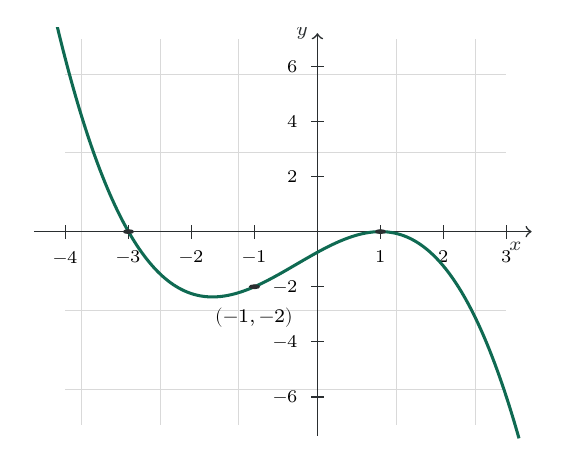
\begin{tikzpicture}[x=8mm,y=3.5mm]
\clip (-4.6,-7.6) rectangle (3.5,7.4);
\draw[black!15,line width=0.3pt] (-4,-7) grid (3,7);
\draw[->,ink,line width=0.6pt] (-4.5,0) -- (3.4,0) node[below left,font=\sffamily\fontsize{7}{8}\selectfont]{$x$};
\draw[->,ink,line width=0.6pt] (0,-7.4) -- (0,7.2) node[left,font=\sffamily\fontsize{7}{8}\selectfont]{$y$};
\foreach \u in {-4,-3,-2,-1,1,2,3}{\draw[ink,line width=0.4pt] (\u,-0.25) -- (\u,0.25); \node[font=\sffamily\fontsize{6.5}{7}\selectfont,below] at (\u+0.0,-0.35){$\u$};}
\foreach \v in {-6,-4,-2,2,4,6}{\draw[ink,line width=0.4pt] (-0.1,\v) -- (0.1,\v); \node[font=\sffamily\fontsize{6.5}{7}\selectfont,left] at (-0.15,\v){$\v$};}
\draw[accent,line width=1.1pt,domain=-4.2:3.2,samples=90,smooth,variable=\xx] plot ({\xx},{-0.25*(\xx+3)*(\xx-1)*(\xx-1)});
\fill[ink] (-1,-2) circle (0.09); \node[font=\sffamily\fontsize{7}{8}\selectfont,anchor=north] at (-1,-2.4){$(-1,-2)$};
\fill[ink] (-3,0) circle (0.09); \fill[ink] (1,0) circle (0.09);
\end{tikzpicture}} The graph crosses the $x$-axis at $x=-3$, touches the $x$-axis at $x=1$, and passes through $(-1,-2)$. Which equation could define $p$?}{$p(x)=\dfrac14(x+3)(x-1)^2$}{$p(x)=-\dfrac14(x+3)(x-1)^2$}{$p(x)=-\dfrac14(x-3)(x+1)^2$}{$p(x)=-\dfrac14(x+3)^2(x-1)$}
\satqa{8}{The function $f$ is defined by \par\vspace{1mm}\centerline{$\displaystyle f(x)=\begin{cases}-2x+9 & \text{if } x<3\\[1mm] (x-5)^2+1 & \text{if } x\ge3\end{cases}$}\vspace{1mm}\par  How many values of $a$ satisfy $f(a)=5$?}{$1$}{$2$}{$3$}{$4$}
\satqa{9}{What is the sum of the zeros of $g(x)=-|x+3|+8$?}{$-11$}{$-6$}{$5$}{$6$}
}
\end{textblock*}
\clearpage
\topicheader{3}{Hard Nonlinear Functions}
\pagefooter{5}
\colrule{32}{238}
\mbox{}%
\begin{textblock*}{\COLW}(\LCOL,32mm)
{\fontsize{10}{12.0}\selectfont
\setkicker{Set 4 (cont.)}{Functions and polynomials}
\satqa{10}{The function $f$ is defined by $f(x)=x^2-6x$. What is the sum of all values of $k$ for which $f(2k)=f(k+3)$?}{$1$}{$3$}{$4$}{$6$}
\satg{11}{The function $g$ is defined by $g(x)=-3x^2+18x-5$. For a real number $a\ne-1$, $g(a)=g(-1)$. What is the value of $a$?}
\satqa{12}{The function $f$ is defined by $f(x)=x^2-2x$, and $g(x)=f(x-2)+3$. How many $x$-intercepts does the graph of $y=g(x)$ have?}{$0$}{$1$}{$2$}{$3$}
\satqa{13}{A parabola opens upward, has $x$-intercepts at $(-2,0)$ and $(6,0)$, and has $y$-intercept $(0,-24)$. Which equation defines the parabola?}{$y=2(x-2)(x+6)$}{$y=-2(x+2)(x-6)$}{$y=(x+2)(x-6)-24$}{$y=2(x+2)(x-6)$}
\satg{14}{The function $f$ is defined by $f(x)=x^2+bx+c$, where $b$ and $c$ are constants. The function $g$ is defined by $g(x)=f(x-4)$ and its zeros are $1$ and $9$. What is the minimum value of $f$?}
\vspace{3mm}\setkicker{Set 5}{Summit: the hardest mixed problems.}
\satqa{1}{The function $f(x)=ax^2+bx+c$ has constants $a$, $b$ and $c$. The graph of $y=f(x)$ is a parabola that opens upward and has vertex $(h,k)$ with $k<0$. Also, $f(-5)=f(1)$. Which of the following must be true?\par\vspace{0.8mm}\hspace*{5mm}I. $b>0$\par\vspace{0.8mm}\hspace*{5mm}II. $c<0$\par\vspace{0.8mm}\hspace*{5mm}III. The equation $f(x)=0$ has two distinct real solutions}{I only}{I and III only}{II and III only}{I, II and III}
}
\end{textblock*}
\begin{textblock*}{\COLW}(\RCOL,32mm)
{\fontsize{10}{12.0}\selectfont
\setkicker{Set 5 (cont.)}{Summit}
\satg{2}{A concert hall sells $1200-30p$ tickets per show when the ticket price is $p$ dollars. The revenue is the price times the number of tickets sold. The owner will not charge less than $\$25$. What is the greatest possible revenue per show, in dollars?}
\satqa{3}{Town A's population $t$ years from now is modeled by $A(t)=12{,}000(1.10)^t$, and town B's is modeled by $B(t)=18{,}000(1.04)^t$. For what least whole number of years $t$ does town A's population first exceed town B's?}{$6$}{$7$}{$8$}{$13$}
\satqa{4}{The number of views $V$ of a video $d$ days after it is posted is modeled by $V(d)=500\cdot2^{d/3}$. Which function gives the number of views $w$ weeks after it is posted?}{$V(w)=500\cdot2^{w/3}$}{$V(w)=500\cdot2^{3w/7}$}{$V(w)=500\cdot2^{21w}$}{$V(w)=500\cdot2^{7w/3}$}
\satg{5}{The table shows values of the quadratic function $f$. \figwrap{\begin{tabular}{|c|c|c|c|}
\hline
\cellcolor{badge!55}\textbf{$x$} & 0 & 1 & 6\\ \hline
\cellcolor{badge!55}\textbf{$f(x)$} & 7 & $-3$ & 7\\ \hline
\end{tabular}} What is the value of $f(4)$?}
\satqa{6}{The graph of $y=g(x)$ is the graph of $y=3^x$ reflected over the $x$-axis, stretched vertically by a factor of $2$, shifted $1$ unit right, and shifted $5$ units up. For what value of $x$ is $g(x)=-49$?}{$3$}{$4$}{$5$}{$28$}
\satg{7}{The function $f$ is defined by $f(x)=3x+k$, where $k$ is a constant. If $f(f(x))=9x+20$ for all $x$, what is the value of $k$?}
}
\end{textblock*}
\clearpage
\topicheader{3}{Hard Nonlinear Functions}
\pagefooter{6}
\colrule{32}{238}
\mbox{}%
\begin{textblock*}{\COLW}(\LCOL,32mm)
{\fontsize{10}{12.0}\selectfont
\setkicker{Set 5 (cont.)}{Summit}
\satqa{8}{The polynomial $p$ is defined by $p(x)=(x-2)(x^2+kx+9)$, where $k$ is a constant. The graph of $y=p(x)$ has exactly two distinct $x$-intercepts. Which of the following could be the value of $k$?}{$6$}{$0$}{$5$}{$10$}
\satqa{9}{The function $f$ is defined by $f(x)=ab^x$, where $a$ and $b$ are constants and $b>0$. If $f(1)=-12$ and $f(3)=-48$, what is the value of $f(0)$?}{$6$}{$-3$}{$-6$}{$-24$}
\satg{10}{A rancher uses $240$ meters of fencing to build a rectangular field and one dividing fence parallel to the field's width. The fencing consists of three pieces of length $W$ meters (the width) and two pieces of length $L$ meters (the length). What is the greatest possible area of the field, in square meters?}
\satqa{11}{A parabola passes through $(-1,10)$, $(0,4)$ and $(3,10)$. Which equation defines it in vertex form?}{$y=2(x+1)^2+2$}{$y=2(x-1)^2+4$}{$y=6(x-1)^2+4$}{$y=2(x-1)^2+2$}
\satqa{12}{The functions $f$ and $g$ are defined by $f(x)=|x-3|$ and $g(x)=2x-5$. For how many values of $x$ is $g(f(x))=f(g(x))$?}{$0$}{$1$}{$2$}{$3$}
\satg{13}{The number of bacteria in a sample grows by $40\%$ every $2$ hours. After $6$ hours, the number of bacteria is what percent greater than the starting number? Enter only the number.}
\satqa{14}{The polynomial $p(x)=a(x+2)(x-3)^2$, where $a>0$, is graphed in the $xy$-plane. For which values of $x$ is $p(x)<0$?}{$x<-2$}{$x>3$}{$-2<x<3$}{$x<-2$ or $x>3$}
}
\end{textblock*}
\begin{textblock*}{\COLW}(\RCOL,32mm)
{\fontsize{10}{12.0}\selectfont
\setkicker{Set 5 (cont.)}{Summit}
\satg{15}{A fish population in a pond is modeled by $P(t)=-2(t-6)^2+130$, where $t$ is the number of months after January 1. For how many months is the population at least $112$ fish?}
\satqa{16}{The graph of $f(x)=2(x-1)^2+3$ is translated $4$ units to the right and then reflected across the $y$-axis to make the graph of $g$. What are the coordinates of the vertex of the graph of $g$?}{$(3,3)$}{$(5,3)$}{$(-3,3)$}{$(-5,3)$}
\satqa{17}{The number of members $N$ of a club $t$ years after it was founded is modeled by $N(t)=800(1.44)^{t/2}$. The number of members grows by what percent each year?}{$20\%$}{$22\%$}{$44\%$}{$120\%$}
\satqa{18}{The table shows values of a function $f$. \figwrap{\begin{tabular}{|c|c|c|c|c|}
\hline
\cellcolor{badge!55}\textbf{$x$} & 1 & 2 & 4 & 5\\ \hline
\cellcolor{badge!55}\textbf{$f(x)$} & 0 & 9 & 45 & 72\\ \hline
\end{tabular}} Which of the following equations defines $f$?}{$f(x)=9x-9$}{$f(x)=3x^2-3$}{$f(x)=3x^2-3x$}{$f(x)=3^{x+1}-9$}
\satqa{19}{The function $f$ is defined by $f(x)=2x^2-3x$, and $g(x)=x-2$. For what value of $x$ is $f(g(x))=f(x)$?}{$7$}{$\dfrac72$}{$\dfrac74$}{$1$}
\satqa{20}{The functions $f$ and $g$ are defined by $f(x)=-(x-2)^2+9$ and $g(x)=2x-4$. At what value of $x$ does $f(g(x))$ reach its maximum?}{$9$}{$3$}{$2$}{$-1$}
}
\end{textblock*}
\clearpage
\topicheader{3}{Hard Nonlinear Functions}
\pagefooter{7}
\mbox{}%
\begin{textblock*}{178mm}(16mm,30mm)
{\bfseries\itshape\color{accent}\fontsize{19}{21}\selectfont\centering Answer Key\par}
\end{textblock*}
\begin{textblock*}{178mm}(16mm,41mm)
{\fontsize{9.5}{12}\selectfont\color{black!70}\centering Multiple choice: the letter. Grid-in: the number to enter. Worked solutions follow on the next pages.\par}
\end{textblock*}
\begin{textblock*}{178mm}(16mm,52mm)
{\fontsize{10}{13}\selectfont
\centering
\setlength{\tabcolsep}{2pt}\renewcommand{\arraystretch}{1.3}
{\sffamily\bfseries\color{accent}\fontsize{11}{13}\selectfont Set 1 \ \textmd{\itshape\small Bridge: read the function before you compute}}\\[1.3mm]
\begin{tabular}{|>{\centering\arraybackslash}p{16mm}|>{\centering\arraybackslash}p{16mm}|>{\centering\arraybackslash}p{16mm}|>{\centering\arraybackslash}p{16mm}|>{\centering\arraybackslash}p{16mm}|>{\centering\arraybackslash}p{16mm}|>{\centering\arraybackslash}p{16mm}|>{\centering\arraybackslash}p{16mm}|>{\centering\arraybackslash}p{16mm}|>{\centering\arraybackslash}p{16mm}|}
\hline
\cellcolor{badge!55}\textbf{1} & \cellcolor{badge!55}\textbf{2} & \cellcolor{badge!55}\textbf{3} & \cellcolor{badge!55}\textbf{4} & \cellcolor{badge!55}\textbf{5} & \cellcolor{badge!55}\textbf{6} & \cellcolor{badge!55}\textbf{7} & \cellcolor{badge!55}\textbf{8} & \cellcolor{badge!55}\textbf{9} & \cellcolor{badge!55}\textbf{10}\\
\hline
\textbf{A} & \textbf{B} & −8 & \textbf{C} & \textbf{D} & 250 & \textbf{A} & \textbf{B} & \textbf{D} & \textbf{C}\\
\hline
\end{tabular}\\[1.5mm]
\begin{tabular}{|>{\centering\arraybackslash}p{16mm}|>{\centering\arraybackslash}p{16mm}|}
\hline
\cellcolor{badge!55}\textbf{11} & \cellcolor{badge!55}\textbf{12}\\
\hline
\textbf{B} & −20\\
\hline
\end{tabular}\\[1.5mm]
\vspace{3.5mm}
{\sffamily\bfseries\color{accent}\fontsize{11}{13}\selectfont Set 2 \ \textmd{\itshape\small Quadratic models, symmetry and equivalent forms}}\\[1.3mm]
\begin{tabular}{|>{\centering\arraybackslash}p{16mm}|>{\centering\arraybackslash}p{16mm}|>{\centering\arraybackslash}p{16mm}|>{\centering\arraybackslash}p{16mm}|>{\centering\arraybackslash}p{16mm}|>{\centering\arraybackslash}p{16mm}|>{\centering\arraybackslash}p{16mm}|>{\centering\arraybackslash}p{16mm}|>{\centering\arraybackslash}p{16mm}|>{\centering\arraybackslash}p{16mm}|}
\hline
\cellcolor{badge!55}\textbf{1} & \cellcolor{badge!55}\textbf{2} & \cellcolor{badge!55}\textbf{3} & \cellcolor{badge!55}\textbf{4} & \cellcolor{badge!55}\textbf{5} & \cellcolor{badge!55}\textbf{6} & \cellcolor{badge!55}\textbf{7} & \cellcolor{badge!55}\textbf{8} & \cellcolor{badge!55}\textbf{9} & \cellcolor{badge!55}\textbf{10}\\
\hline
\textbf{A} & 1875 & \textbf{C} & \textbf{D} & 32 & \textbf{A} & \textbf{D} & \textbf{B} & \textbf{C} & \textbf{D}\\
\hline
\end{tabular}\\[1.5mm]
\begin{tabular}{|>{\centering\arraybackslash}p{16mm}|>{\centering\arraybackslash}p{16mm}|>{\centering\arraybackslash}p{16mm}|>{\centering\arraybackslash}p{16mm}|}
\hline
\cellcolor{badge!55}\textbf{11} & \cellcolor{badge!55}\textbf{12} & \cellcolor{badge!55}\textbf{13} & \cellcolor{badge!55}\textbf{14}\\
\hline
20 & \textbf{A} & \textbf{C} & 7\\
\hline
\end{tabular}\\[1.5mm]
\vspace{3.5mm}
{\sffamily\bfseries\color{accent}\fontsize{11}{13}\selectfont Set 3 \ \textmd{\itshape\small Exponential models: factors, rates and two-point rebuilds}}\\[1.3mm]
\begin{tabular}{|>{\centering\arraybackslash}p{16mm}|>{\centering\arraybackslash}p{16mm}|>{\centering\arraybackslash}p{16mm}|>{\centering\arraybackslash}p{16mm}|>{\centering\arraybackslash}p{16mm}|>{\centering\arraybackslash}p{16mm}|>{\centering\arraybackslash}p{16mm}|>{\centering\arraybackslash}p{16mm}|>{\centering\arraybackslash}p{16mm}|>{\centering\arraybackslash}p{16mm}|}
\hline
\cellcolor{badge!55}\textbf{1} & \cellcolor{badge!55}\textbf{2} & \cellcolor{badge!55}\textbf{3} & \cellcolor{badge!55}\textbf{4} & \cellcolor{badge!55}\textbf{5} & \cellcolor{badge!55}\textbf{6} & \cellcolor{badge!55}\textbf{7} & \cellcolor{badge!55}\textbf{8} & \cellcolor{badge!55}\textbf{9} & \cellcolor{badge!55}\textbf{10}\\
\hline
\textbf{D} & \textbf{B} & 1500 & \textbf{C} & \textbf{A} & \textbf{B} & 15 & \textbf{D} & \textbf{C} & \textbf{B}\\
\hline
\end{tabular}\\[1.5mm]
\begin{tabular}{|>{\centering\arraybackslash}p{16mm}|>{\centering\arraybackslash}p{16mm}|>{\centering\arraybackslash}p{16mm}|>{\centering\arraybackslash}p{16mm}|}
\hline
\cellcolor{badge!55}\textbf{11} & \cellcolor{badge!55}\textbf{12} & \cellcolor{badge!55}\textbf{13} & \cellcolor{badge!55}\textbf{14}\\
\hline
18 & \textbf{A} & \textbf{C} & 80\\
\hline
\end{tabular}\\[1.5mm]
\vspace{3.5mm}
{\sffamily\bfseries\color{accent}\fontsize{11}{13}\selectfont Set 4 \ \textmd{\itshape\small Composition, transformations, polynomials and piecewise rules}}\\[1.3mm]
\begin{tabular}{|>{\centering\arraybackslash}p{16mm}|>{\centering\arraybackslash}p{16mm}|>{\centering\arraybackslash}p{16mm}|>{\centering\arraybackslash}p{16mm}|>{\centering\arraybackslash}p{16mm}|>{\centering\arraybackslash}p{16mm}|>{\centering\arraybackslash}p{16mm}|>{\centering\arraybackslash}p{16mm}|>{\centering\arraybackslash}p{16mm}|>{\centering\arraybackslash}p{16mm}|}
\hline
\cellcolor{badge!55}\textbf{1} & \cellcolor{badge!55}\textbf{2} & \cellcolor{badge!55}\textbf{3} & \cellcolor{badge!55}\textbf{4} & \cellcolor{badge!55}\textbf{5} & \cellcolor{badge!55}\textbf{6} & \cellcolor{badge!55}\textbf{7} & \cellcolor{badge!55}\textbf{8} & \cellcolor{badge!55}\textbf{9} & \cellcolor{badge!55}\textbf{10}\\
\hline
−6 & \textbf{B} & \textbf{D} & \textbf{C} & −11 & \textbf{A} & \textbf{B} & \textbf{C} & \textbf{B} & \textbf{C}\\
\hline
\end{tabular}\\[1.5mm]
\begin{tabular}{|>{\centering\arraybackslash}p{16mm}|>{\centering\arraybackslash}p{16mm}|>{\centering\arraybackslash}p{16mm}|>{\centering\arraybackslash}p{16mm}|}
\hline
\cellcolor{badge!55}\textbf{11} & \cellcolor{badge!55}\textbf{12} & \cellcolor{badge!55}\textbf{13} & \cellcolor{badge!55}\textbf{14}\\
\hline
7 & \textbf{A} & \textbf{D} & −16\\
\hline
\end{tabular}\\[1.5mm]
\vspace{3.5mm}
{\sffamily\bfseries\color{accent}\fontsize{11}{13}\selectfont Set 5 \ \textmd{\itshape\small Summit: the hardest mixed problems}}\\[1.3mm]
\begin{tabular}{|>{\centering\arraybackslash}p{16mm}|>{\centering\arraybackslash}p{16mm}|>{\centering\arraybackslash}p{16mm}|>{\centering\arraybackslash}p{16mm}|>{\centering\arraybackslash}p{16mm}|>{\centering\arraybackslash}p{16mm}|>{\centering\arraybackslash}p{16mm}|>{\centering\arraybackslash}p{16mm}|>{\centering\arraybackslash}p{16mm}|>{\centering\arraybackslash}p{16mm}|}
\hline
\cellcolor{badge!55}\textbf{1} & \cellcolor{badge!55}\textbf{2} & \cellcolor{badge!55}\textbf{3} & \cellcolor{badge!55}\textbf{4} & \cellcolor{badge!55}\textbf{5} & \cellcolor{badge!55}\textbf{6} & \cellcolor{badge!55}\textbf{7} & \cellcolor{badge!55}\textbf{8} & \cellcolor{badge!55}\textbf{9} & \cellcolor{badge!55}\textbf{10}\\
\hline
\textbf{B} & 11250 & \textbf{C} & \textbf{D} & −9 & \textbf{B} & 5 & \textbf{A} & \textbf{C} & 2400\\
\hline
\end{tabular}\\[1.5mm]
\begin{tabular}{|>{\centering\arraybackslash}p{16mm}|>{\centering\arraybackslash}p{16mm}|>{\centering\arraybackslash}p{16mm}|>{\centering\arraybackslash}p{16mm}|>{\centering\arraybackslash}p{16mm}|>{\centering\arraybackslash}p{16mm}|>{\centering\arraybackslash}p{16mm}|>{\centering\arraybackslash}p{16mm}|>{\centering\arraybackslash}p{16mm}|>{\centering\arraybackslash}p{16mm}|}
\hline
\cellcolor{badge!55}\textbf{11} & \cellcolor{badge!55}\textbf{12} & \cellcolor{badge!55}\textbf{13} & \cellcolor{badge!55}\textbf{14} & \cellcolor{badge!55}\textbf{15} & \cellcolor{badge!55}\textbf{16} & \cellcolor{badge!55}\textbf{17} & \cellcolor{badge!55}\textbf{18} & \cellcolor{badge!55}\textbf{19} & \cellcolor{badge!55}\textbf{20}\\
\hline
\textbf{D} & \textbf{A} & 174.4 & \textbf{A} & 6 & \textbf{D} & \textbf{A} & \textbf{B} & \textbf{C} & \textbf{B}\\
\hline
\end{tabular}\\[1.5mm]
\vspace{3.5mm}
}
\end{textblock*}
\clearpage
%%AUTOFLOW-SOLUTIONS
\newgeometry{top=34mm,bottom=24mm,left=16mm,right=16mm}
\pagestyle{solstyle}
\setlength{\columnsep}{14mm}\setlength{\columnseprule}{0.4pt}
{\fontsize{10}{13.6}\selectfont
\begin{multicols}{2}
\solkicker{Set 1}{Worked solutions}
\solitem{1}{A ($9$)}{In $a(x-h)^2+k$ with $a<0$ the maximum value is $k=9$ (it happens at $x=-4$). The traps: $-4$ is where the maximum happens, $4$ is the sign slip on $h$, and $-2$ is just $a$.}{Vertex form reads h and k}
\solitem{2}{B (The car's value drops by $15\%$ each year.)}{Each year the value is multiplied by $0.85=1-0.15$, so it drops by $15\%$. (Choice $85\%$ confuses the factor with the rate; $0.85\%$ forgets to convert a decimal to a percent.)}{Growth factor = 1 ± rate}
\solitem{3}{Ans. −8}{Inside first: $g(1)=3$. Then $f(3)=9-12-5=-8$. (Doing $g(f(1))$ instead gives $-15$.)}{Compose inside-out}
\solitem{4}{C ($3$)}{The zeros are $3$ (double), $-1$ and $6$. Distinct intercepts: $3$. (Choice 4 counts the double root twice; choice 2 counts only the places where the graph crosses.)}{Zeros and multiplicity}
\solitem{5}{D ($g(x)=(x+3)^2-2$)}{Left $3$ means $f(x+3)$ (inside, opposite sign); down $2$ means $-2$ outside. So $g(x)=(x+3)^2-2$.}{Shift rules (x → x − h)}
\solitem{6}{Ans. 250}{The axis is $x=-\dfrac{60}{2(-2)}=15$. Then $P(15)=-450+900-200=250$.}{Vertex = max/min}
\solitem{7}{A ($12$)}{$f(0)=5a=-15$, so $a=-3$. The axis is $x=\frac{1+5}2=3$ and $f(3)=-3(2)(-2)=12$. (Traps: $-15$ is $f(0)$, $3$ is where the maximum happens, $-12$ is a sign slip.)}{Axis = midpoint of the zeros}
\solitem{8}{B (The amount is cut in half every $6$ hours.)}{$\left(\frac12\right)^{t/6}$ multiplies by $\frac12$ each time $t$ grows by $6$: a half-life of $6$ hours. The initial amount is $A(0)=400$.}{Per-period exponent}
\solitem{9}{D ($21$)}{The axis is $x=3$, so the minimum is $f(3)=18-36+c=c-18=3$ and $c=21$. (Traps: $12$ forgets the factor $2$, $18$ is just the constant part, $3$ is the minimum itself.)}{Vertex = max/min}
\solitem{10}{C ($8$)}{$|x-4|=5$, so $x=9$ or $x=-1$, and the sum is $8$. (Traps: $5$ is only $|x-4|$, $10$ is the difference of the solutions, $4$ is the center.)}{Absolute value: two cases}
\solitem{11}{B ($4x^2+12x+8$)}{Put $f(x)$ inside $g$: $(2x+3)^2-1=4x^2+12x+9-1$. (Traps: $2x^2+1$ is $f(g(x))$; $4x^2+8$ squares the terms one by one; $4x^2+12x+9$ forgets the $-1$.)}{Compose inside-out}
\solitem{12}{Ans. −20}{$p(0)=a(2)(-1)(-4)=8a=16$, so $a=2$. Then $p(3)=2(5)(2)(-1)=-20$.}{Zeros and multiplicity}
\solkicker{Set 2}{Worked solutions}
\solitem{1}{A}{The axis is $t=-\frac{24}{2(-4)}=3$ and $h(3)=-36+72+10=46$, so $(3,46)$ is the vertex: the maximum height is $46$ ft at $t=3$. (The other choices swap the coordinates, call the vertex the landing point, or call $46$ the starting height; the starting height is $h(0)=10$.)}{Interpret the model}
\solitem{2}{Ans. 1875}{$R(p)=p(300-12p)$ has zeros $p=0$ and $p=25$, so its maximum is halfway at $p=12.5$: $R=12.5(300-150)=12.5\cdot150=1875$.}{Optimize: vertex of the product}
\solitem{3}{C ($800$)}{The side along the wall is $80-2w$, so $A=w(80-2w)$ with zeros $0$ and $40$. The maximum is at $w=20$: $A=20\cdot40=800$. (Traps: $20$ is $w$; $400$ treats the pen as a square with 4 fenced sides; $1600$ is $40^2$.)}{Optimize: vertex of the product}
\solitem{4}{D ($3(x+3)^2-7$)}{$3(x^2+6x)+20=3\big[(x+3)^2-9\big]+20=3(x+3)^2-27+20=3(x+3)^2-7$. (Forgetting to multiply the $9$ by $3$ gives $+11$; skipping the correction gives $+20$.)}{Complete the square}
\solitem{5}{Ans. 32}{$g(1)=g(7)$ puts the axis at $x=4$, so $g(x)=a(x-4)^2-18$. Then $g(0)=16a-18=14$ gives $a=2$, and $g(-1)=2(25)-18=32$.}{Symmetry about the axis}
\solitem{6}{A (I only)}{$f(-2)=f(6)$ puts the axis at $x=2$, so $-\frac b{2a}=2$ and $b=-4a$. With $a<0$ that gives $b>0$: I is true. Only $c=f(0)>0$ is known, so $c>b$ can fail (take $a=-3$, $b=12$, $c=1$): II is not forced.}{Symmetry about the axis}
\solitem{7}{D ($-3$)}{$f(1)=f(3)$, so the axis is $x=2$. With $f(x)=a(x-2)^2+k$: $f(1)=a+k=-1$ and $f(0)=4a+k=5$, so $a=2$, $k=-3$. The minimum is $-3$. (The table's $-1$ is not the lowest point; $2$ is where the minimum happens.)}{Symmetry about the axis}
\solitem{8}{B ($70$)}{Solve $-0.5x^2+40x-350=0$: $x^2-80x+700=0$, so $x=10$ or $x=70$. Profit is $\ge0$ for $10\le x\le70$, so the largest output is $70$. (Traps: $10$ is the smaller zero, $40$ the vertex, $80$ the sum of the zeros.)}{Axis = midpoint of the zeros}
\solitem{9}{C ($5$)}{$f(x)>0$ means $(x-4)^2<9$, so $1<x<7$: the integers $2,3,4,5,6$ give $5$. (Counting $\ge0$ gives $7$; $3$ is the half-width; $9$ is $k$.)}{Vertex form reads h and k}
\solitem{10}{D ($y=2(x+2)^2+5$)}{$y=a(x+2)^2+5$ and $y(0)=4a+5=13$ give $a=2$. (Check the vertex, not only the point: $2(x-2)^2+5$ also passes through $(0,13)$ but has vertex $(2,5)$; $(x+2)^2+9$ has vertex $(-2,9)$.)}{Vertex form reads h and k}
\solitem{11}{Ans. 20}{The vertex is at $t=\frac b{10}$, so the maximum is $2+\frac{b^2}{20}=22$. Then $b^2=400$ and $b=20$ (positive).}{Vertex = max/min}
\solitem{12}{A ($10$)}{The minimum of $f$ is $f(3)=k-9$. The graph stays above $y=-2$ only if $k-9>-2$, i.e. $k>7$. Only $10$ works. ($k=7$ makes the vertex touch the line.)}{Vertex = max/min}
\solitem{13}{C ($1<x<3$)}{$-3(x-1)(x-3)>0$. The parabola opens downward, so it is above the axis between the zeros: $1<x<3$. (The outside-the-zeros choice is for an upward parabola.)}{Factor and sketch}
\solitem{14}{Ans. 7}{Equal outputs at $x=0$ and $x=2$ put the axis at $x=1$. Write $y=a(x-1)^2+k$: $a+k=6$ and $16a+k=-9$, so $a=-1$ and $k=7$.}{Symmetry about the axis}
\solkicker{Set 3}{Worked solutions}
\solitem{1}{D ($1.5\%$)}{Each month multiplies by $1.2^{1/12}\approx1.0153$, about $1.5\%$ growth. (Dividing $20\%$ by $12$ gives the trap $1.7\%$; $20\%$ is the yearly rate; $240\%$ multiplies by $12$.)}{Unit change: t = m/12}
\solitem{2}{B ($5.3$)}{In $12$ hours there are $\frac{12}5=2.4$ doubling periods, so the factor is $2^{2.4}\approx5.3$. (Traps: $2.4$ is the number of periods; $4.0$ rounds the periods down to $2$; $24$ is $12\cdot2$.)}{Per-period exponent}
\solitem{3}{Ans. 1500}{From $t=2$ to $t=6$ the population is multiplied by $4$ in $4$ hours, so $b^4=4$ and $b^2=2$. Going back from $t=2$ to $t=0$ divides by $b^2=2$: $3000\div2=1500$.}{Two points: divide to get b}
\solitem{4}{C ($f(x)=2(3)^x$)}{Divide: $\frac{ab^5}{ab^2}=b^3=\frac{486}{18}=27$, so $b=3$. Then $a\cdot3^2=18$ gives $a=2$. (Choice 27 is $b^3$, not $b$; $18$ is $f(2)$, not $f(0)$; $6$ divides by $b$ only once.)}{Two points: divide to get b}
\solitem{5}{A}{The exponent $\frac t3$ counts blocks of $3$ years; each block multiplies by $1.5$, i.e. a $50\%$ increase. (The yearly factor is $1.5^{1/3}\approx1.145$, not $1+\frac{0.5}3$.)}{Per-period exponent}
\solitem{6}{B ($3$)}{$f(x)>0$ means $2^x<\frac{50}6\approx8.33$, so $x\le3$ (since $2^3=8$). The positive integers $1,2,3$ give $3$. (Counting $x=0$ gives $4$; using $2^x<8$ strictly gives $2$; $8$ is a value of $2^x$.)}{Graph it (Desmos)}
\solitem{7}{Ans. 15}{Solve $1.05^t>2$: graph $y=1.05^t$ and $y=2$; they cross near $t\approx14.2$. Since $1.05^{14}\approx1.98<2$ and $1.05^{15}\approx2.08$, the answer is $15$.}{Graph it (Desmos)}
\solitem{8}{D ($320(0.5)^x$)}{$g(x)=40(0.5)^{x-3}=40(0.5)^{-3}(0.5)^x=40\cdot8\,(0.5)^x=320(0.5)^x$. (Using $0.5^{+3}$ gives $5$; $-3$ outside is a vertical shift; $0.125$ is $0.5^3$, a changed base.)}{Shift rules (x → x − h)}
\solitem{9}{C ($15{,}625$)}{Over $4$ years the factor is $\frac{12500}{8000}=\frac{25}{16}$, so $b^4=\frac{25}{16}$ and $b^2=\frac54$. In $6$ years (three blocks of $2$): $8000\left(\frac54\right)^3=15{,}625$. (Traps: $14{,}750$ is linear growth; $19{,}531$ applies the 4-year factor again; $30{,}518$ uses $25\%$ per year.)}{Two points: divide to get b}
\solitem{10}{B ($5000\left(\sqrt[3]{2}\right)^t$)}{$2^{t/3}=\left(2^{1/3}\right)^t$: the base becomes the cube root of $2$. (Traps: $8=2^3$, $\frac23$ and $6$ come from mishandling the exponent $\frac t3$.)}{Per-period exponent}
\solitem{11}{Ans. 18}{There are $\frac{20}8=2.5$ half-life periods, so the fraction left is $\left(\frac12\right)^{2.5}\approx0.1768$, i.e. about $18\%$.}{Per-period exponent}
\solitem{12}{A ($11$)}{$3(2)^x=12$ gives $2^x=4$, so $p=2$. $q=g(0)=3-12=-9$. Then $p-q=2+9=11$. (Traps: $-7$ is $p+q$, $-11$ is $q-p$, $9$ is $|q|$.)}{Intercepts: set x = 0 or y = 0}
\solitem{13}{C ($30$)}{$T(0)=a+20=100$, so $a=80$ (the room temperature $20$ is the floor, not part of $a$). Then $T(3)=80\cdot\frac18+20=30$. (Traps: $12.5=100\cdot\frac18$; $32.5$ uses $a=100$; $60$ halves only once.)}{Intercepts: set x = 0 or y = 0}
\solitem{14}{Ans. 80}{At $x=2$: $5\cdot4=20$ and $c\left(\frac12\right)^2=\frac c4$. Setting $20=\frac c4$ gives $c=80$.}{Substitute the point}
\solkicker{Set 4}{Worked solutions}
\solitem{1}{Ans. −6}{$f(g(x))=2x^2-8x+3$ and $g(f(x))=(2x+3)^2-4(2x+3)=4x^2+4x-3$. Setting them equal: $2x^2+12x-6=0$, so the sum of the solutions is $-\frac{12}2=-6$.}{Compose inside-out}
\solitem{2}{B ($1$)}{Compute both orders. $x=1$: $f(g(1))=f(2)=1$, $g(f(1))=g(3)=3$. $x=2$: $f(g(2))=f(4)=2$, $g(f(2))=g(1)=2$ (equal). $x=3$: $f(3)=4$ but $g(4)=1$. $x=4$: $f(1)=3$ but $g(2)=4$. Only $x=2$ works. (Choice 4 assumes the order does not matter.)}{Compose inside-out}
\solitem{3}{D $(1,11)$}{$f$ has vertex $(2,-3)$. $f(x+1)$ moves it left $1$: $(1,-3)$. Multiplying by $-2$ gives $y=6$, and adding $5$ gives $11$: vertex $(1,11)$. (Traps: $(3,11)$ shifts right; $(1,2)$ forgets the $-2$; $(1,1)$ subtracts the $5$.)}{Shift rules (x → x − h)}
\solitem{4}{C ($5.5$)}{$g(x)=0$ when $2x-4=-2$ or $2x-4=5$, so $x=1$ or $x=4.5$ and the sum is $5.5$. (Plugging the zeros forward, $2(-2)-4$ and $2(5)-4$, gives the trap $-2$; ignoring the factor $2$ gives $11$; $3$ is the sum of the zeros of $f$.)}{Shift rules (x → x − h)}
\solitem{5}{Ans. −11}{$f(x-5)$ moves the maximum point to $(8,7)$. Multiplying by $-3$ turns it into a minimum at $y=-21$, and adding $2$ gives $y=-19$. So $(h,k)=(8,-19)$ and $h+k=-11$.}{Shift rules (x → x − h)}
\solitem{6}{A}{The factor $(x-3)^2$ has an even exponent, so the graph touches the axis at $3$ without crossing. The degree is $4$ (even) and the leading coefficient $-2$ is negative, so both ends point down.}{Leading coefficient and ends}
\solitem{7}{B ($p(x)=-\dfrac14(x+3)(x-1)^2$)}{A crossing at $-3$ is a single factor and a touch at $1$ is a squared factor: $p(x)=a(x+3)(x-1)^2$. Using $p(-1)=a(2)(4)=-2$ gives $a=-\frac14$. (The other choices have the signs or the double root in the wrong place, or give $p(-1)=+2$.)}{Zeros and multiplicity}
\solitem{8}{C ($3$)}{Branch 1 ($a<3$): $-2a+9=5$ gives $a=2$, valid. Branch 2 ($a\ge3$): $(a-5)^2=4$ gives $a=3$ or $a=7$, both valid ($a=3$ belongs to this branch). Three values: $2,3,7$.}{Pick the branch}
\solitem{9}{B ($-6$)}{$|x+3|=8$ gives $x=5$ or $x=-11$, and the sum is $-6$ (it is twice the center $-3$). (Traps: $5$ or $-11$ is a single zero; $6$ comes from using the center $+3$.)}{Absolute value: two cases}
\solitem{10}{C ($4$)}{Equal outputs happen when the inputs are equal ($2k=k+3$, so $k=3$) or symmetric about the axis $x=3$ ($2k+k+3=6$, so $k=1$). The sum is $4$. (Choices $3$ and $1$ each find only one of the two cases; $6$ is the sum of the symmetric inputs.)}{Symmetry about the axis}
\solitem{11}{Ans. 7}{The axis is $x=-\frac{18}{2(-3)}=3$. The point symmetric to $x=-1$ is $2(3)-(-1)=7$.}{Symmetry about the axis}
\solitem{12}{A ($0$)}{$g(x)=(x-2)^2-2(x-2)+3=x^2-6x+11$, with discriminant $36-44<0$. (Also: $f$ has vertex $(1,-1)$, so $g$ has vertex $(3,2)$, above the axis and opening up: no intercepts. Choice 2 assumes $g$ keeps the zeros of $f$.)}{Shift rules (x → x − h)}
\solitem{13}{D ($y=2(x+2)(x-6)$)}{$y=a(x+2)(x-6)$ and $y(0)=-12a=-24$ give $a=2>0$. (Traps: $(x-2)(x+6)$ has the zeros at the wrong signs; $-2(\ldots)$ opens downward; subtracting $24$ shifts the whole graph instead of scaling it.)}{Test the points}
\solitem{14}{Ans. −16}{$g(x)=f(x-4)=0$ at $x=1,9$ means $f(-3)=f(5)=0$ (subtract $4$ from each zero). So $f(x)=(x+3)(x-5)$, the axis is $x=1$ and the minimum is $f(1)=4(-4)=-16$.}{Shift rules (x → x − h)}
\solkicker{Set 5}{Worked solutions}
\solitem{1}{B (I and III only)}{$f(-5)=f(1)$ puts the axis at $x=-2$, so $-\frac b{2a}=-2$ and $b=4a>0$ (I is true). The vertex is below the axis and the parabola opens up, so it crosses the axis twice (III is true). But $c=f(0)=4a+k$ can be positive (try $a=5$, $k=-1$), so II is not forced.}{Symmetry about the axis}
\solitem{2}{Ans. 11250}{$R(p)=p(1200-30p)$ has zeros $0$ and $40$, so its vertex is $p=20$, which is below the allowed minimum $25$. For $p\ge25$ the revenue only falls, so the best price is $25$: $R=25(450)=11{,}250$. (The vertex value $12{,}000$ is not allowed.)}{Domain limit: check the vertex}
\solitem{3}{C ($8$)}{Graph both curves: they cross where $\left(\frac{1.10}{1.04}\right)^t=1.5$, near $t\approx7.2$. At $t=7$, $A\approx23{,}385<B\approx23{,}687$; at $t=8$, $A\approx25{,}723>B\approx24{,}634$. So $t=8$. (Traps: $6$ is the gap $10-4$; $7$ rounds $7.2$ down; $13$ is $\frac{50}{4}$.)}{Graph it (Desmos)}
\solitem{4}{D ($V(w)=500\cdot2^{7w/3}$)}{$w$ weeks is $d=7w$ days. Substitute: $500\cdot2^{7w/3}$. (Traps: leaving $d=w$; inverting $7$ and $3$; multiplying $3\cdot7$.)}{Unit change: t = m/12}
\solitem{5}{Ans. −9}{$f(0)=f(6)$ puts the axis at $x=3$. Write $f(x)=a(x-3)^2+k$: $9a+k=7$ and $4a+k=-3$, so $a=2$, $k=-11$. Then $f(4)=2(1)-11=-9$.}{Symmetry about the axis}
\solitem{6}{B ($4$)}{The transformations give $g(x)=-2\cdot3^{x-1}+5$. Then $-2\cdot3^{x-1}=-54$, so $3^{x-1}=27=3^3$ and $x-1=3$, $x=4$. (Traps: $3$ forgets the right shift; $5$ shifts the wrong way; $28$ treats $3^{x-1}$ as $x-1$ added to $27$.)}{Shift rules (x → x − h)}
\solitem{7}{Ans. 5}{$f(f(x))=3(3x+k)+k=9x+4k$. Then $4k=20$ and $k=5$. (Squaring $f$ or adding $k$ only once are the usual slips.)}{Compose inside-out}
\solitem{8}{A ($6$)}{The quadratic factor must add exactly one new zero: a double root ($D=k^2-36=0$, so $k=\pm6$; for $k=6$ the root is $-3$). For $k=0$ or $5$ it has no real zeros (one intercept in all); for $k=10$ it has two new zeros (three intercepts).}{Zeros and multiplicity}
\solitem{9}{C ($-6$)}{$b^2=\frac{-48}{-12}=4$, so $b=2$. Going back one step from $f(1)$ divides by $b$: $f(0)=\frac{-12}2=-6$. (Traps: $-24$ multiplies by $b$; $-3$ divides by $b^2$; $6$ loses the sign.)}{Two points: divide to get b}
\solitem{10}{Ans. 2400}{With width $W$, $3W+2L=240$, so $L=\frac{240-3W}2$ and $A=\frac{W(240-3W)}2$. The zeros are $W=0$ and $W=80$, so the maximum is at $W=40$: $L=60$ and $A=2400$.}{Optimize: vertex of the product}
\solitem{11}{D ($y=2(x-1)^2+2$)}{Equal outputs at $x=-1$ and $x=3$ put the axis at $x=1$. Then $y=a(x-1)^2+k$: $a+k=4$ and $4a+k=10$, so $a=2$, $k=2$. (Sign slip on $h$ gives $2(x+1)^2$; the others fail $(0,4)$.)}{Vertex form reads h and k}
\solitem{12}{A ($0$)}{$g(f(x))=2|x-3|-5$ and $f(g(x))=|2x-8|=2|x-4|$. The equation becomes $|x-3|-|x-4|=2.5$, but the left side always lies between $-1$ and $1$. Graphing $y=2|x-3|-5$ and $y=2|x-4|$ shows two V shapes with the second always at least $3$ units above the first: they never meet, so there are $0$ solutions.}{Graph it (Desmos)}
\solitem{13}{Ans. 174.4}{$6$ hours is $3$ periods of $2$ hours: $1.4^3=2.744$, which is $174.4\%$ greater. (Not $3\cdot40=120\%$: growth compounds.)}{Growth factor = 1 ± rate}
\solitem{14}{A ($x<-2$)}{The factor $(x-3)^2$ is never negative, so the sign is the sign of $(x+2)$ (with $a>0$), except at the touching zero $x=3$. So $p<0$ only for $x<-2$. (The graph does not change sign at $x=3$.)}{Zeros and multiplicity}
\solitem{15}{Ans. 6}{$-2(t-6)^2+130\ge112$ gives $(t-6)^2\le9$, so $3\le t\le9$. By symmetry the period is $2\cdot3=6$ months long.}{Vertex form reads h and k}
\solitem{16}{D $(-5,3)$}{Vertex $(1,3)$; right $4$: $(5,3)$; reflect across the $y$-axis: $(-5,3)$. (Reflecting first and then shifting right gives $(-1+4,3)=(3,3)$, the order trap.)}{Shift rules (x → x − h)}
\solitem{17}{A ($20\%$)}{$1.44^{t/2}=\left(\sqrt{1.44}\right)^t=1.2^t$, so the yearly factor is $1.2$: a $20\%$ increase. (Traps: $44\%$ is the growth per $2$ years; $22\%$ halves it; $120\%$ is the factor, not the increase.)}{Per-period exponent}
\solitem{18}{B ($f(x)=3x^2-3$)}{Test each equation at all four points. $3x^2-3$ gives $0,9,45,72$ at $x=1,2,4,5$. (The linear choice fits only $x=1,2$; $3x^2-3x$ fails at $x=2$; the exponential fails at $x=2$.)}{Test the points}
\solitem{19}{C ($\dfrac74$)}{$f$ has axis $x=\frac34$. $f(x-2)=f(x)$ means $x-2$ and $x$ are symmetric about it: $(x-2)+x=\frac32$, so $x=\frac74$. (Or expand: $-8x+14=0$.) (Traps: $\frac72$ forgets to halve; $7$ drops the denominator.)}{Symmetry about the axis}
\solitem{20}{B ($3$)}{$f(g(x))=-(2x-6)^2+9$ is maximal when $2x-6=0$, i.e. $g(x)=2$ (the input where $f$ peaks), so $x=3$. (Traps: $2$ is where $f$ peaks; $9$ is the maximum value; $-1$ solves $2x+4=2$.)}{Compose inside-out}
\end{multicols}}
\end{document}
